\documentclass[aspectratio=169]{beamer}
\usepackage[UTF8,heading,fontset=none]{ctex} % 中文支持
\usepackage{ncepu-beamer} % 应用主题

\usepackage{color}
\usepackage{amsmath}
\usepackage{tikz}        % 绘图
\usepackage{minted}      % 代码高亮
\usepackage{subcaption}  % 创建子图
\usepackage{algorithm2e} % 伪代码

% --------------- 字体设置 --------------- %
%% 配置方式见 README.md
%% 如果不想使用自定义字体,可以注释掉下面的设置
%% 并且删除 ctex 包的 `fontset=none` 选项
\usepackage{fontspec}
\setmainfont{HarmonyOS Sans}
\setsansfont{HarmonyOS Sans}
\setmonofont{CodeNewRoman Nerd Font}
\setCJKmainfont{HarmonyOS Sans SC}
\setCJKsansfont{HarmonyOS Sans SC}
\setCJKmonofont{HarmonyOS Sans SC}
% --------------- 字体设置 --------------- %

% --------------- svg 设置 --------------- %
\usepackage[notransparent]{svg} % 插入 svg 矢量图
\setsvg{
  %% 设置 inkscape 路径(inkscape 用于处理 svg 矢量图)
  inkscapeexe={"C:/Program Files/Inkscape/bin/inkscape.com"}, % Windows
  % inkscapeexe={"/usr/bin/inkscape"}, % Linux
  %% 设置 svg 文字随图片缩放
  inkscapelatex=false
}
%% NOTE: draw.io 中的文本需要关闭自动换行和格式化文本
% --------------- svg 设置 --------------- %

% 输入信息
\title{科研题目}
\subtitle{副标题} % 不需要副标题可以直接删掉
\author{报告人}
\institute{控制与计算机工程学院}
\date{\today}

\begin{document}

\begin{frame}[noframenumbering]

  \titlepage

\end{frame}

\begin{frame}{目录}

  \centering
  \begin{minipage}{0.8\textwidth}
    \tableofcontents
  \end{minipage}

\end{frame}

% 从这里开始你的创作

\section{这是第一部分}

\begin{frame}{图文分列}

  \begin{columns}
    \column{0.4\textwidth}

    这是有编号的列表:
    \begin{enumerate}
      \item 使用 columns 环境
      \item 使用 column 命令调整比例
      \item 这里是一个插入 svg 矢量图的例子
    \end{enumerate}

    \column{0.6\textwidth}

    \begin{figure}
      \centering
      \includesvg[width=\textwidth]{img/example_img.svg}
      \caption{这里写图片的名字}
    \end{figure}

  \end{columns}

\end{frame}

\section{这是第二部分}

\subsection{这是第二部分的第一小节}

\begin{frame}{frame 的主标题\footnote{标题脚注}}{frame 的副标题}

  这是一个嵌套列表:

  \begin{itemize}
    \item 111
    \item 222
    \item 333\footnote{这里有一条脚注}
      \begin{itemize}
        \item 3.111
        \item 3.222\footnote{这里还有一条脚注}
      \end{itemize}
  \end{itemize}

\end{frame}

\subsection{这是第二部分的第二小节}

\begin{frame}{写点数学公式}

  当观察次数 $n \rightarrow \infty$ 时,表示在单位时间内持续观察用户提交任务的过程:

  \begin{equation*}
    \begin{split}
      P\left\{X=k\right\} & = \lim_{n \rightarrow \infty} C_n^k \, p^k (1-p)^{n-k}                                                                                                                              \\
      & = \lim_{n \rightarrow \infty} \frac{n(n-1)\dots(n-(k-1))}{k!} \left(\frac{\lambda}{n}\right)^k \left(1-\frac{\lambda}{n}\right)^{n-k}                                               \\
      & = \frac{\lambda^k}{k!} \lim_{n \rightarrow \infty} \frac{n(n-1)\dots(n-(k-1))}{n^k} \left(1-\frac{\lambda}{n}\right)^{-k} \colorbox{yellow}{$\left(1-\frac{\lambda}{n}\right)^{n}$} \\
      & = \frac{\lambda^k}{k!} \colorbox{yellow}{$e^{-\lambda}$}
    \end{split}
  \end{equation*}

  此时单位时间内\textcolor{blue}{实际}提交的任务数量 $X$ 服从泊松分布 $X \sim P(\lambda)$ 。

\end{frame}

\subsection{这是第二部分的第三小节}

\begin{frame}{block 示例}

  记 $[0,t]$ 时间段内用户提交的任务数量为 $N(t)$ ,$(s,t]$ 时间段内用户提交的任务数量为 $N(s,t] = N(t) - N(s)$ 。

  \begin{block}{泊松过程}
    \begin{itemize}
      \item $N(0)=0$:初始时刻没有用户提交任务
      \item 独立增量性:在互不相交的时间段内,用户提交任务的数量相互独立
      \item 平稳增量性:在长度相等的时间段 $t$ 内,任务提交数量服从相同的概率分布 $P(\lambda t)$
    \end{itemize}
  \end{block}

  因此 $\forall s, N(s,s+t] \sim P(\lambda t)$ :
  $$P\left\{N(s,s+t]=k\right\} = \frac{(\lambda t)^k}{k!} e^{-\lambda t}$$

\end{frame}

\section{这是第三部分}

\subsection{使用 tikz 绘制图形}

\begin{frame}{用 tikz 画了个图}{这部分内容放在了另外一个 tex 文件中}

    代码默认存在 $10$ 台虚拟机,输入状态 $s_t$ 为当前提交任务的类型和 $10$ 台虚拟机的 $T_{idle}$ :
    $$s_t = \left[Type,\, T_{idle}^{(1)},\, T_{idle}^{(2)},\, \dots,\, T_{idle}^{(10)}\right]^T$$

    DQN输出在当前状态 $s_t$ 下,对分配到每台虚拟机的总共 $10$ 个动作的评分。

    \begin{figure}
        \begin{tikzpicture}[scale=0.2,font=\small]
            \draw[->] (-4,0) node[left] {$s_t$} -- (-0.5,0);

            \draw[step=1cm] (0,-4) grid (1,4);
            \node[below] at (0.5,-4) {输入层 $x \in \mathbb{R}^{11}$};

            \draw[->] (1.5,0) -- (16.5,0);
            \node[above right] at (1.5,0) {$ReLU(W_1^Tx+b_1)$};

            \draw[step=1cm] (17,-6) grid (18,6);
            \node[below] at (17.5,-6) {隐藏层 $y \in \mathbb{R}^{20}$};

            \draw[->] (18.5,0) -- (27.5,0);
            \node[above right] at (18.5,0) {$W_2^T y+b_2$};

            \draw[step=1cm] (28,-3) grid (29,3);
            \node[below] at (28.5,-3) {输出层 $q \in \mathbb{R}^{10}$};
        \end{tikzpicture}
    \end{figure}

    其中两层全连接层的参数:$W_1 \in \mathbb{R}^{11 \times 20},\, b_1 \in \mathbb{R}^{20},\, W_2 \in \mathbb{R}^{20 \times 10},\, b_2 \in \mathbb{R}^{10}$ 。
\end{frame}

\subsection{使用 tikz 绘制子图}

\begin{frame}{用 tikz 花了两个子图}

    \begin{figure}
        \centering

        \begin{subfigure}[c]{0.4\textwidth}
            \begin{tikzpicture}
                \draw[->] (0,0) node[below] {$0$} -- (5,0) node[right] {$t$};

                \draw[-] (1,3pt) -- (1,-3pt) node[below] {$W_1$};
                \draw[-] (3.5,3pt) -- (3.5,-3pt) node[below] {$W_2$};

                \node[above] at (2.25,7pt) {$T_2$};
                \draw[<->] (1,5pt) -- (3.5,5pt);

                \node[below=1.5em] at (1,0) {$s$};
                \draw[dashed] (4,0) -- (4,-1.5em) node[below] {$s+t$};
            \end{tikzpicture}

            \caption{$T_2 \leqslant t$}
        \end{subfigure}
        \qquad
        \begin{subfigure}[c]{0.4\textwidth}
            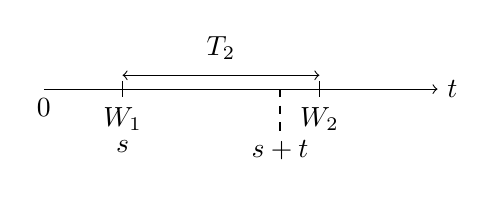
\begin{tikzpicture}
                \draw[->] (0,0) node[below] {$0$} -- (5,0) node[right] {$t$};

                \draw[-] (1,3pt) -- (1,-3pt) node[below] {$W_1$};
                \draw[-] (3.5,3pt) -- (3.5,-3pt) node[below] {$W_2$};

                \node[above] at (2.25,7pt) {$T_2$};
                \draw[<->] (1,5pt) -- (3.5,5pt);

                \node[below=1.5em] at (1,0) {$s$};
                \draw[dashed] (3,0) -- (3,-1.5em) node[below] {$s+t$};
            \end{tikzpicture}

            \caption{$T_2 > t$}
        \end{subfigure}
    \end{figure}

\end{frame}


\section{这是第四部分}

\begin{frame}[fragile]{试试代码高亮}{记得加 fragile 参数}

  这个字是正常大小

  \scriptsize
  \begin{minted}{python3}
        # scriptsize 命令变成脚本大小
        # 生成时间间隔
        intervalT = stats.expon.rvs(scale=1 / lamda, size=self.jobNum)
        # 对时间间隔累加得到提交时间
        self.arrival_Times = np.around(intervalT.cumsum(), decimals=3)
  \end{minted}

  \normalsize
  又恢复了正常大小

  \scriptsize
  \begin{minted}{python3}
        # 又变成了脚本大小
        self.jobsMI = np.random.normal(self.jobMI, self.jobMI_std, self.jobNum)
        self.jobsMI = self.jobsMI.astype(int)
  \end{minted}

\end{frame}

\section{这是第五部分}

\begin{frame}[shrink=5]{最后试试伪代码}{shrink 参数调整 frame 的缩小系数}

  \scriptsize % 字太大了调小点
  \begin{algorithm}[H]
    \SetAlgoLined
    设定环境参数、DRL超参数,随机初始化DQN参数,赋予target网络相同的参数\;
    \ForEach{Episode}{
      重置环境\;
      \ForEach{Step}{
        对于状态 $s_t$ 根据 $\epsilon$-greedy 策略得到动作 $a_t$\;
        执行动作 $a_t$ 后环境变为 $s_{t+1}$ 并得到奖励 $r_t$\;
        将轨迹 $(s_t, a_t, r_t, s_{t+1})$ 存入replay memory\;
        \If{Step $>$ 开始学习步数}{
          从replay memory中随机抽取 $30$ 个样本作为minibatch\;
          \ForEach{sample in minibatch}{
            将 $s_t$ 传入Q-network得到 $a_t$ 对应的 $Q_{value}$\;
            将 $s_{t+1}$ 传入target-network得到输出的最大值 $Q_{target}$\;
            根据损失函数 $Loss = (Q_{value} - (r_t + \gamma \cdot Q_{target}))^2$ 使用梯度下降法更新Q-network\;
          }
          \If{Step \% 50 = 0}{
            使用Q-network的参数更新target-network\;
          }
          减小 $\epsilon$\;
        }
      }
    }
  \end{algorithm}

\end{frame}

\begin{frame}

  \centering
  \Huge
  \usefont{OT1}{pzc}{m}{n}
  Thanks for listening!

\end{frame}

\end{document}
